\documentclass[a4paper]{report}

%====================== PACKAGES ======================

\usepackage[french]{babel}
\usepackage[utf8x]{inputenc}
%pour gérer les positionnement d'images
\usepackage{float}
\usepackage{amsmath}
\usepackage{graphicx}
\usepackage[colorinlistoftodos]{todonotes}
\usepackage{url}
%pour les informations sur un document compilé en PDF et les liens externes / internes
\usepackage{hyperref}
%pour la mise en page des tableaux
\usepackage{array}
\usepackage{tabularx}
%pour utiliser \floatbarrier
%\usepackage{placeins}
%\usepackage{floatrow}
%espacement entre les lignes
\usepackage{setspace}
%modifier la mise en page de l'abstract
\usepackage{abstract}
%police et mise en page (marges) du document
\usepackage[T1]{fontenc}
\usepackage[top=2cm, bottom=2cm, left=2cm, right=2cm]{geometry}
%Pour les galerie d'images
\usepackage{subfig}
\usepackage{multirow}

%====================== INFORMATION ET REGLES ======================

%rajouter les numérotation pour les \paragraphe et \subparagraphe
\setcounter{secnumdepth}{4}
\setcounter{tocdepth}{4}

\hypersetup{							% Information sur le document
pdfauthor = {Rémy ZIRNHELD,
			Alban MANZANO,
			Florian GRANTE,
    		Nicolas BONNET},			% Auteurs
pdftitle = {Rubik'INT -
			Solveur de Rubik's cube},			% Titre du document
pdfsubject = {Livrable 1},		% Sujet
pdfkeywords = {rubikscube, tsp, informatique},	% Mots-clefs
pdfstartview={FitH}}					% ajuste la page à la largueur de l'écran

%======================== DEBUT DU DOCUMENT ========================

\begin{document}

%régler l'espacement entre les lignes
\newcommand{\HRule}{\rule{\linewidth}{0.5mm}}

%page de garde
\begin{titlepage}
\begin{center}

% Upper part of the page. The '~' is needed because only works if a paragraph has started.

\includegraphics[width=0.35\textwidth]{./logo}~\\[1cm]

\textsc{\LARGE PRO3600 - Projet informatique}\\[1.5cm]

\textsc{\Large }\\[0.5cm]

% Title
\HRule \\[0.4cm]

{\huge \bfseries Rubik'INT\\
Solveur de Rubik's Cube \\[0.4cm] }

\HRule \\[1.5cm]

% Author and supervisor
\begin{minipage}{0.4\textwidth}
\begin{flushleft} \large
\emph{Auteurs:}\\
Rémy \textsc{ZIRNHELD}\\
Alban \textsc{MANZANO}\\
Florian \textsc{GRANTE}\\
Nicolas \textsc{BONNET}
\end{flushleft}
\end{minipage}
\begin{minipage}{0.4\textwidth}
\begin{flushright} \large
\emph{Tutrice:} \\
Amina \textsc{GUERMOUCHE}
\end{flushright}
\end{minipage}

\vfill

% Bottom of the page
{\large \today}

\end{center}
\end{titlepage}


%ne pas numéroter cette page
\thispagestyle{empty}
%\newpage

%%%\input{./abstract.tex}

\tableofcontents
\thispagestyle{empty}
\setcounter{page}{0}
%ne pas numéroter le sommaire

%\newpage

%espacement entre les lignes d'un tableau
\renewcommand{\arraystretch}{1.5}

%====================== INCLUSION DES PARTIES ======================

~
\thispagestyle{empty}
%recommencer la numérotation des pages à "1"
\setcounter{page}{0}
\newpage

\chapter*{Introduction}
\addcontentsline{toc}{chapter}{Introduction}

Le projet de développement informatique nous a offert l'opportunité de créer le programme que nous voulions.
Divers sujets se présentaient à nous. Nous étions déterminés à trouver un projet nous permettant de mettre en œuvre plusieurs domaines de l'informatique.
Nous avons choisi le Rubik's Cube, un casse-tête fascinant: il s'agit d'un cube constitué de 3x3x3 sous-cubes colorés pouvant tourner selon trois axes.
Le Rubik's Cube se distingue par l'immense complexité de sa résolution contrastant avec sa simplicité apparente.
Chaque personne capable de résoudre le cube doit suivre une méthodologie stricte et faire preuve d'une certaine intuition.
L'objectif derrière le choix de ce célèbre casse-tête en tant que sujet est d'apprendre des domaines de l'informatique qui sont nouveau pour nous.

Le défi que nous nous sommes lancés est d'apprendre à une machine à résoudre ce casse-tête.
Pour cela nous devrons nous confronter à plusieurs problématiques.
La première, la plus évidente, est sa résolution. Nous allons avoir besoin de faire appel à des connaissances mathématiques et algorithmiques\cite{cite1}
De plus nous voulons donner un aspect pratique à notre projet. Ainsi, l'utilisateur devra pouvoir réussir à résoudre son cube grâce au programme.
Il est donc indispensable d'élaborer une interface utilisateur.
Nous devrons aussi ajouter une solution simple pour reconnaître la configuration du cube dans le programme. Nous utiliserons un algorithme de \textit{computer vision} sur un flux vidéo acquis en temps réel par une webcam.
Ainsi, ce projet regroupe les thématiques de la création d'interface utilisateur, de l'algorithmie et du traitement d'image.



\chapter{Cahier des charges}
\section{Premier prototype}
Il s'agit premièrement d'implémenter la fonction basique de notre programme: la résolution du cube. Nous allons donc lui fournir en entrée un fichier contenant les couleurs de toutes les facettes du cube. Le programme cherchera à le résoudre et renverra les mouvements nécessaires à sa résolution. Par exemple en utilisant la notation de Singmaster\cite{cite11}.
Différentes méthodes sont pour l'instant envisagées:
\begin{itemize}
    \item La première consiste à implémenter un algorithme de résolution simple: par exemple le premier algorithme généralement appris par les humains.\cite{cite2} Le principe de celui-ci est d'envisager la résolution dans l'ordre suivant: d'abord une face, puis la première couronne, la seconde couronne et enfin la dernière face\cite{cite2}. Pour résoudre le Rubik's Cube de cette manière, le programme devra être capable de reconnaître la configuration dans laquelle se trouve le cube à un moment donné et lui
    appliquer une procédure, c'est-à-dire une suite prédéfinie de rotations. Les autres méthodes utilisées par les humains reposent sur ce même principe avec différentes configurations et procédures. Dans le cas des méthodes dites avancées, c'est-à-dire permettant de résoudre le Rubik's Cube en un plus petit nombre de rotations, le nombre de configurations et de procédures à apprendre augmente drastiquement.
\item Un algorithme reposant sur une machine de Boltzmann\cite{cite10} est également envisagée. Cet algorithme aurait une fonction d'évaluation de l'énergie du cube (plus le cube est proche de sa résolution, plus son énergie est faible) et chercherait à minimiser cette énergie via des rotations aléatoires ou des procédures aléatoires. Ces procédures auraient d'autant plus de chances d'être choisie que leur action réduit l'énergie du cube. Cet algorithme pourrait être utilisé conjointement avec le premier pour la résolution.
\item Un troisième algorithme dit en deux phases consiste à utiliser un algorithme A*\cite{cite3} (parcours d'un arbre en profondeur amélioré par une heuristique) pour placer les angles du cube au bon endroit lors de la première phase. La seconde phase consiste à utiliser réduire le nombre des rotations possibles à un groupe de cardinal plus petit.\footnote{Plus d'information sur les groupes du cube \cite{cite12}} Cet algorithme permet de résoudre le Rubik's Cube en une vingtaine de coups, mais est également plus dur à implémenter\cite{cite0}. Cet
    algorithme est une amélioration d'un algorithme passant par 5 groupes\cite{cite4}.
\end{itemize}

\section{L'affichage en 3D}
La prochaine étape du développement consiste à faire une interface homme machine. Il faut que l'utilisateur puisse visualiser les étapes successives de résolution du Rubik's Cube. Pour cela nous comptons afficher une fenêtre avec un bouton pour aller à l'étape suivante et une image en 3D de la configuration du cube que l'utilisateur devrait avoir dans les mains.

\section{\textit{Computer vision}}
Une fois que l'affichage a été réalisé, il faut pouvoir permettre de rentrer la configuration du cube au départ. Pour cela nous présenterons les différentes faces du cube à la caméra et un algorithme de traitement d'image\footnote{L'algorithme pourra être réalisé grâce à la bibliothèque OpenCV\cite{cite7}} sera capable de reconstituer le cube virtuellement.



 
\chapter{Interface}
\section{Affichage 3D}
Nos recherches sur la façon de réaliser un rendu 3D en Java nous a amené à utiliser une bibliothèque : \textit{Java3D}\cite{cite5}.
Même si le rendu à un instant t est satisfaisant (voir image ci-dessous), il ne nous permet pas, du moins de façon optimisée, de réaliser des animations comme la rotation du cube, le rendu étant figé une fois affiché.
\begin{figure}[h]
\begin{center}
	\makebox[\textwidth]{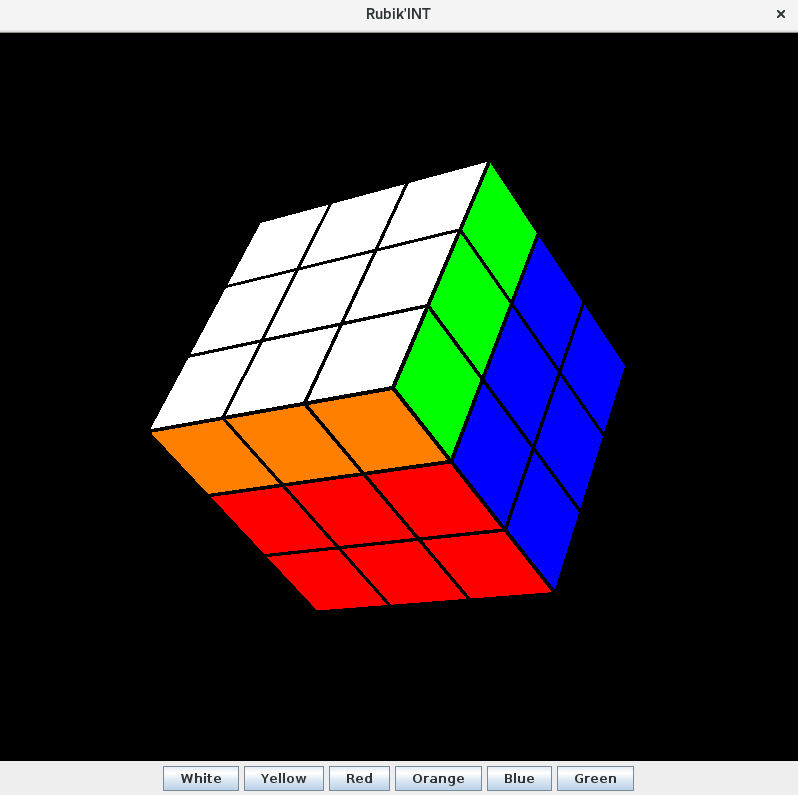
\includegraphics[width=.4\paperwidth]{diagrammes/rendu3D.png}}
\end{center}
\caption{GUI}
\end{figure}
Cet essai nous a permis de mieux cerner notre besoin. 
Il est nécessaire d'avoir un rendu 3D dans lequel l'objet affiché reste modifiable, dans notre cas de pouvoir réaliser les animation de rotation du cube. C'est pourquoi nous avons finalement décidé de réaliser tout cela à l'aide de la bibliothèque : \textit{OpenGL}\cite{cite6}.

\section{Interface fenêtrée}
Cet affichage 3D devra être intégré dans une interface, il sera accompagné de boutons pour rendre notre programme de résolution autonome et facile d'utilisation. Nous pouvons voir une ébauche d'utilisation de la bibliothèque \textit{Swing}\cite{cite9} sur la photo ci-dessus. L'objectif de cette première fenêtre est de faire tourner la face du cube de la couleur associée au bouton lorsque l'utilisateur clique dessus.

À terme, l'interface sera scindée en trois parties selon la logique suivante :

\begin{itemize}
    \item Un accueil pour que l'utilisateur puisse choisir la façon dont il veut résoudre son Rubik's cube (avec ou sans prise de photo d'un vrai cube)
    \item Une interface permettant la prise de photo du cube et donc de récupérer sa configuration 
    \item Une interface pour la résolution du cube.
\end{itemize}
Notre objectif est de rendre l'interface le plus \textit{user-friendly} possible.




\chapter{Résoudre un Rubik's cube}

\section{Modéliser un Rubik's Cube}

Dans ce projet, nous nous sommes rendu compte que modéliser un Rubik's Cube était moins trivial qu'il n'en avait l'air.
Le modèle qu'on cherchait devait respecter plusieurs critères. 
\begin{enumerate}
    \item Premièrement nous devions avoir une interface pour récupérer la couleur de chaque facette à tout moment.
    \item Ensuite il fallait qu'on ait une fonction qui simule une rotation sur une couronne quelquonque.
    \item Enfin, notre modélisation devait être assez efficace pour permettre une résolution qui ne prenne pas trop de temps.
\end{enumerate}
\subsection{Les premières idées naïves}

\subsubsection{Le tableau de facettes}
La première idée qui nous est venue est de stocker la couleur de chaque facette dans un tableau.
Cette méthode n'est pas très efficace: créer une fonction pour simuler la rotation d'une couronne s'avère être compliqué.
De plus la complexité en mémoire n'est pas très bonne.

\subsubsection{La liste chaînée}
Similairement à cette première méthode, nous avons également songé à stocker les couleurs dans une liste chaînée en 2 dimensions.
On aurait "mis à plat" le Rubik's Cube et on aurait parcouru ses facettes sur un plan infini.

\subsubsection{Les cubies}
La deuxième idée que nous avons eu était de considérer les \textit{cubies}, petits cube constituant le Rubik's Cube en 3x3x3.
La rotation semblait être plus facile car nous aurions pu travailler avec des transformations d'angles et de position dans l'espace.
Cependant cette méthode faisait apparaître des complications d'implémentations rendant notre code très lourd.

\subsection{Le tableau de permutations}
Nous avons finalement décidé d'adopter une approche plus mathématique : le tableau de permutations.

Cela consiste en un tableau de 6*8=48 cases (six faces et 8 facettes qui peuvent bouger).
Le Rubik's résolu est alors représenté par un tableau rempli de 0 à 47 (dans l'ordre).
Effectuer une rotation est alors équivalent à appliquer une permutation sur le tableau.
Cela s'implémente simplement et l'algorithme est efficace.
Retrouver la couleur en fonction du numéro dans la case du tableau est aisé en définissant les permutations.

\begin{figure}[h]
\begin{center}
    \makebox[\textwidth]{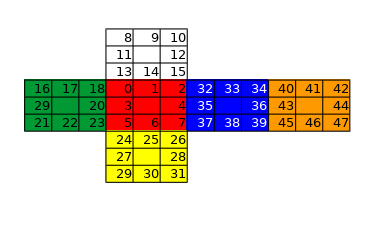
\includegraphics[width=.5\paperwidth]{diagrammes/perm.png}}
\end{center}
    \caption{Les permutations du Rubik's}
\end{figure}

C'est finalement cette approche que nous avons décidé de garder car elle nous permettait de garder un code simple et efficace.

\section{Algorithme de résolution}
Une fois que nous avons créé un objet représentant le cube que nous pouvions manipuler virtuellement, nous nous sommes attaqué à la partie résolution.
Résoudre un Rubik's Cube nécessite d'être rigoureux et surtout méthodique.
C'est donc pourquoi nous avions initialement pensé qu'un ordinateur serait parfaitement adapté pour appliquer une méthode de résolution.
Cependant, nous nous sommes aperçu que il y a toujours une partie 



\newpage

%récupérer les citation avec "/footnotemark"
\nocite{*}

%choix du style de la biblio
\bibliographystyle{plain}
%inclusion de la biblio
\bibliography{bibliographie.bib}
%voir wiki pour plus d'information sur la syntaxe des entrées d'une bibliographie

\end{document}
